\documentclass[conference]{IEEEtran}
\IEEEoverridecommandlockouts
% The preceding line is only needed to identify funding in the first footnote. If that is unneeded, please comment it out.
\usepackage{cite}
\usepackage{amsmath,amssymb,amsfonts}
\usepackage{algorithmic}
\usepackage{graphicx}
\usepackage{textcomp}
\usepackage{xcolor}
\def\BibTeX{{\rm B\kern-.05em{\sc i\kern-.025em b}\kern-.08em
    T\kern-.1667em\lower.7ex\hbox{E}\kern-.125emX}}
\begin{document}

\title{The Road to the Complete Larval Drosophila Connectome}

\author{\IEEEauthorblockN{Anatol Nica}
\IEEEauthorblockA{\textit{......}\\
\textit{........}\\
.....}
}

\maketitle

\begin{abstract}
..........................................................
\end{abstract}

\begin{IEEEkeywords}
......................
\end{IEEEkeywords}

\section{Introduction}

Understanding how the brain processes information remains an important
challenge in neuroscience and computer science. Neurons communicate
through complex networks of connections, and studying these connections
can help researchers investigate how neural circuits support behavior.
A connectome represents the connections between neurons within a nervous
system or a defined part of it.

The fruit fly, Drosophila melanogaster, has become an important
model organism for connectomics because of its relatively compact nervous
system and the availability of advanced imaging and computational
techniques. Its larval stage is particularly interesting because it
provides opportunities to investigate neural development, sensory
processing, and motor behavior.

Early studies focused on relatively small neuronal circuits and
specific brain regions. As imaging technologies and reconstruction
methods improved, researchers became able to identify larger numbers
of neurons and their synaptic connections. These developments gradually
expanded the scale of available datasets, making it possible to study
neural networks in greater detail.

An important step in this progress was the reconstruction of larval
neuronal circuits containing approximately 3,000 neurons. Subsequent
research expanded the available anatomical and connectivity information,
providing increasingly comprehensive descriptions of neural systems.
These advances also introduced new computational challenges, including
the storage, processing, visualization, and interpretation of large
connectivity datasets.

This topic connects neuroscience with computer science through image
processing, graph representation, data analysis, and computational
reconstruction. Reviewing the development of larval Drosophila
connectomics can therefore provide a clearer understanding of how
technical progress has changed the scale and scope of neural circuit
research.

This work will 
.................................................

\section{Main Problem}

Although connectomics has progressed considerably, the development
of a comprehensive neural connectivity map has required overcoming
several technical and methodological difficulties. The reconstruction
of neurons from electron microscopy images is a demanding process
because neuronal structures are densely packed, branches overlap,
and synaptic connections can be difficult to identify accurately.

One major problem is the scale of reconstruction. Early studies
could investigate individual neurons, small circuits, or selected
regions of the nervous system. Larger reconstructions require the
identification and tracing of many more neurons, together with their
synapses and associated anatomical information. Increasing the size
of a dataset consequently increases the computational resources and
validation effort required.

Another challenge is the reliability of reconstructed connections.
Errors in tracing neuronal branches or identifying synapses can affect
the resulting connectivity graph. Automated methods can accelerate
reconstruction, but they do not eliminate the need for quality control
and correction. Differences in imaging techniques, annotation
procedures, and dataset coverage can also make comparisons between
studies difficult.

A further issue concerns the meaning of completeness. A dataset may
cover a particular brain region, a collection of neural circuits, or
a much larger portion of the nervous system. These datasets should
not automatically be treated as equivalent. Their coverage, resolution,
biological stage, and available annotations must be considered when
comparing progress across different studies.

For larval Drosophila connectomics, an important question is how
research progressed from relatively small reconstructions to more
comprehensive neural connectivity datasets. Understanding this
progress requires examining not only the number of reconstructed
neurons but also the imaging technologies, reconstruction methods,
and research objectives behind each milestone.

The main problem addressed in this work is 

..............................................

\section{Possible Approach}

This assignment begins with a quantitative literature review of the larval
\textit{Drosophila melanogaster} connectome. The research idea is historical:
to trace how advances in electron-microscopy imaging, image processing,
neuron reconstruction, and validation made increasingly large-scale larval
connectome projects possible. The systematic review will identify these
milestones, compare their reported scale and coverage, and summarize the
remaining barriers to a more complete connectome.

\subsection{Scope and Objectives}

The preliminary question is: \textit{How did imaging and reconstruction
methods develop to make large-scale larval \textit{D. melanogaster}
connectomics possible, and how did the scale and coverage of the resulting
datasets change?} Quantitative measures include publication counts and,
where reported in eligible studies, image volume, reconstructed neurons,
synapses, and brain-region coverage. The reported 2015--2024 period is a
retrospective filter of the existing 2010--2026 exports, not a new search.
The Scopus API log is dated 4 November 2026. The exact date and query history
for the direct Web of Science (WoS) website search were not retained.

The target records are primary studies on larval \textit{D. melanogaster}
connectivity and connectome datasets, including the imaging, image
processing, reconstruction, synapse identification, and validation methods
that enabled them. Reviews may inform background reading but will not count
as primary studies. The current exports contain multiple publication types
and no verified document-type filter, so this criterion still requires
screening.

\subsection{Search Terms and Query Design}

The initial keyword matrix groups terms by concept. These terms were found
in the existing Scopus searches and should be checked against the IEEE
Taxonomy, ACM Computing Classification System, and database subject terms
before the final search is run.

\begin{table}[htbp]
\caption{Initial keyword matrix}
\label{tab:keywords}
\centering
\footnotesize
\begin{tabular}{|p{0.20\linewidth}|p{0.70\linewidth}|}
\hline
\textbf{Concept} & \textbf{Candidate terms and variants} \\
\hline
Organism & \textit{Drosophila melanogaster}; drosophila; ``fruit fly'' \\
\hline
Life stage & larva; larvae; larval \\
\hline
Connectivity & connectome; connectomic; ``synaptic connectivity'';
``wiring diagram''; ``neural circuit''; ``neuronal circuit'' \\
\hline
Data and methods & ``electron microscopy''; ``serial section'';
``volume EM''; neuron reconstruction; circuit reconstruction \\
\hline
\end{tabular}
\end{table}

Within each concept block, related terms are combined with OR; concept
blocks are combined with AND. Three query variants cover connectome terms,
microscopy/reconstruction, and neural circuits. The field-neutral Boolean
expressions are listed in \texttt{search.txt}; the Scopus script maps them
to the database field syntax and applies the 2010--2026 publication-year
filter. Scopus returned 142, 378, and 57 results for the three queries
(577 query results including overlap), which produced 488 unique Scopus
records. The researcher searched WoS directly on its website and exported
the three \texttt{savedrecs} files. The exact WoS interface query and date
remain undocumented, so the search should be rerun and logged before the
review is considered systematic and complete.

\subsection{Screening and Preliminary Results}

\begin{table}[htbp]
\caption{Source records and deduplication (2015--2024)}
\label{tab:source-counts}
\centering
\scriptsize
\begin{tabular}{|p{0.40\linewidth}|r|r|r|}
\hline
\textbf{Source export} & \textbf{Records} & \textbf{Duplicates} & \textbf{Retained} \\
\hline
Scopus API & 340 & 1 & 339 \\
WoS \texttt{savedrecs (7).xls} & 79 & 69 & 10 \\
WoS \texttt{savedrecs (8).xls} & 116 & 81 & 35 \\
WoS \texttt{savedrecs (9).xls} & 33 & 33 & 0 \\
\hline
\textbf{Total} & \textbf{568} & \textbf{184} & \textbf{384} \\
\hline
\end{tabular}
\end{table}

The 184 duplicates were matched by DOI. The Scopus export has abstracts for
269 of its 340 records in this period. Missing abstracts were looked up
manually where accessible, as reported by the researcher; per-record source
provenance was not retained. The final merged screening set has 343
abstracts (89.3\%) and 41 missing abstracts (10.7\%).

\begin{table}[htbp]
\caption{Preliminary screening counts (2015--2024)}
\label{tab:screening-counts}
\centering
\footnotesize
\begin{tabular}{|l|r|r|}
\hline
\textbf{Stage or label} & \textbf{Records} & \textbf{Percent} \\
\hline
Possible inclusion (preliminary label) & 21 & 5.5\% \\
Exclude (preliminary label) & 354 & 92.2\% \\
Unclear (preliminary label) & 9 & 2.3\% \\
\hline
Abstract available & 343 & 89.3\% \\
Abstract missing & 41 & 10.7\% \\
\hline
\end{tabular}
\end{table}

Annual record counts were 31, 32, 39, 43, 39, 39, 39, 52, 34, and 36 for
2015 through 2024, respectively. The largest annual count was 52 in 2022
(13.5\% of the 384 records), followed by 43 in 2018 (11.2\%). Scopus citation
metadata are available for 339 records: these records have 10,213 citations
in total (mean 30.1; median 18), an h-index of 52, and 226 records with at
least 10 citations. These citation figures are a preliminary export snapshot;
its retrieval date was not recorded. Author/index keywords are present for
178 records (46.4\%). After case-folding but before synonym normalization,
``Drosophila'' occurs 59 times and ``expression'' 24 times; variants such as
``Drosophila melanogaster'' and ``Drosophila-melanogaster'' must be normalized
before interpreting keyword trends.

The INCLUDE/EXCLUDE/UNCLEAR decisions are preliminary. The 21 possible
inclusions and 9 unclear records require full-text assessment. The source,
deduplication, and screening totals reconcile. Aggregate extraction outputs,
query logs, criteria, and scripts are available in the project repository
\cite{repo}; raw database exports and record-level abstracts are excluded.

\subsection{Proposed Connectome Research Pipeline}

The project is a systematic review of the historical development of larval
connectomics, not a planned graph-ablation experiment. After search and
screening, the review will extract milestones in electron-microscopy
acquisition, image alignment and segmentation, neuron and synapse
reconstruction, and validation. Reported dataset scale and coverage will be
compared quantitatively where the source studies provide comparable
measures. The synthesis will explain how these technical advances enabled
larger reconstructions and identify limitations that remain on the path
toward a more complete connectome. The current screening counts are
preliminary; historical extraction and synthesis remain to be completed.

\begin{figure*}[!t]
\centering
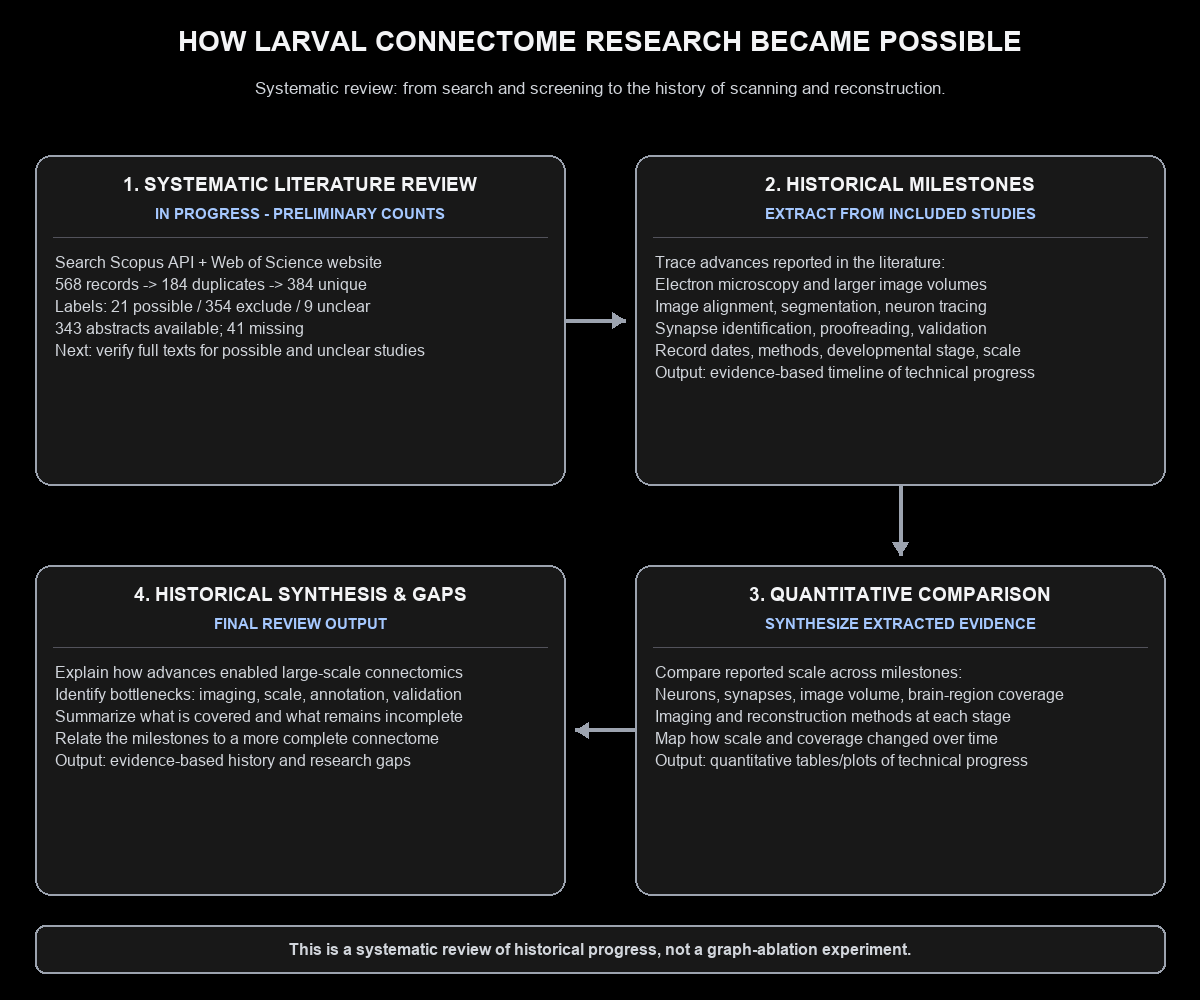
\includegraphics[width=0.95\textwidth]{pipe.png}
\caption{Systematic-review workflow for tracing historical technical
advances that enabled larval connectome imaging and reconstruction.}
\label{fig:workflow}
\end{figure*}
\begin{thebibliography}{00}
\bibitem{repo} A. Nica, ``The Road to the Complete Larval Drosophila Connectome,'' GitHub repository. [Online]. Available: \texttt{https://github.com/NicaAnatol/The-Road-to-the-Complete-Larval-Drosophila-Connectome}
\end{thebibliography}
\end{document}